
\documentclass[11pt]{article}

\usepackage[a4paper, margin=1in]{geometry}
\usepackage[utf8]{inputenc}
\usepackage{geometry}
\usepackage{graphicx}
\usepackage{url}
\usepackage{array}
\usepackage{hyperref}
\usepackage[table,dvipsnames]{xcolor}
\usepackage{afterpage}
\usepackage{fix-cm}
\usepackage{lipsum}
\usepackage{sectsty}
\usepackage{tikz}

\usepackage{multirow}
\usepackage{longtable}
\usepackage{caption}

\captionsetup[figure]{
    justification=centering
}

\definecolor{UoDBlue}{RGB}{67, 101, 226}
\definecolor{UoDDarkBlue}{RGB}{61, 88, 151}
\definecolor{UoDLightBlue}{RGB}{209,226,242}

\usepackage{fontspec}
\setromanfont{BaxterSans}[
    Path=./Baxter/,
    Extension = .otf,
    UprightFont=*-Regular,
    BoldFont=*-Bold,
    ItalicFont=*-RegularItalic,
    BoldItalicFont=*-BoldItalic
    ]
    
\sectionfont{\color{UoDBlue}}
\subsectionfont{\color{UoDBlue}}

\begin{document}

\captionsetup[table]{skip=10pt}


\newgeometry{top=20mm, left=10mm, bottom=20mm} 
\pagecolor{UoDDarkBlue}\afterpage{\nopagecolor}


\includegraphics[width=9cm]{logo2.png}
\vspace*{1cm}

\noindent \fontsize{50}{55}\selectfont \textcolor{white}{\textbf{Optimising the Dublin Bikes}}
\fontsize{50}{55}\selectfont \textcolor{white}{\textbf{Grid using Machine Learning}}

\vspace{15mm}
\noindent \Large\textcolor{white}{\textbf{Group 5 Report}}

\vspace{15mm}

\Large
\noindent\textcolor{white}{Kaley Burg}
\newline \textcolor{white}{Niall Carty}
\newline \textcolor{white}{Sara Cid}
\thispagestyle{empty}

\vspace*{\fill} 
\begin{tikzpicture}[remember picture, overlay]
    \clip (current page.south west) -- ++(\paperwidth, 13cm) -- ++(0, -15cm) -- cycle;
    \node[inner sep=0pt, anchor=south west] at (current page.south west) {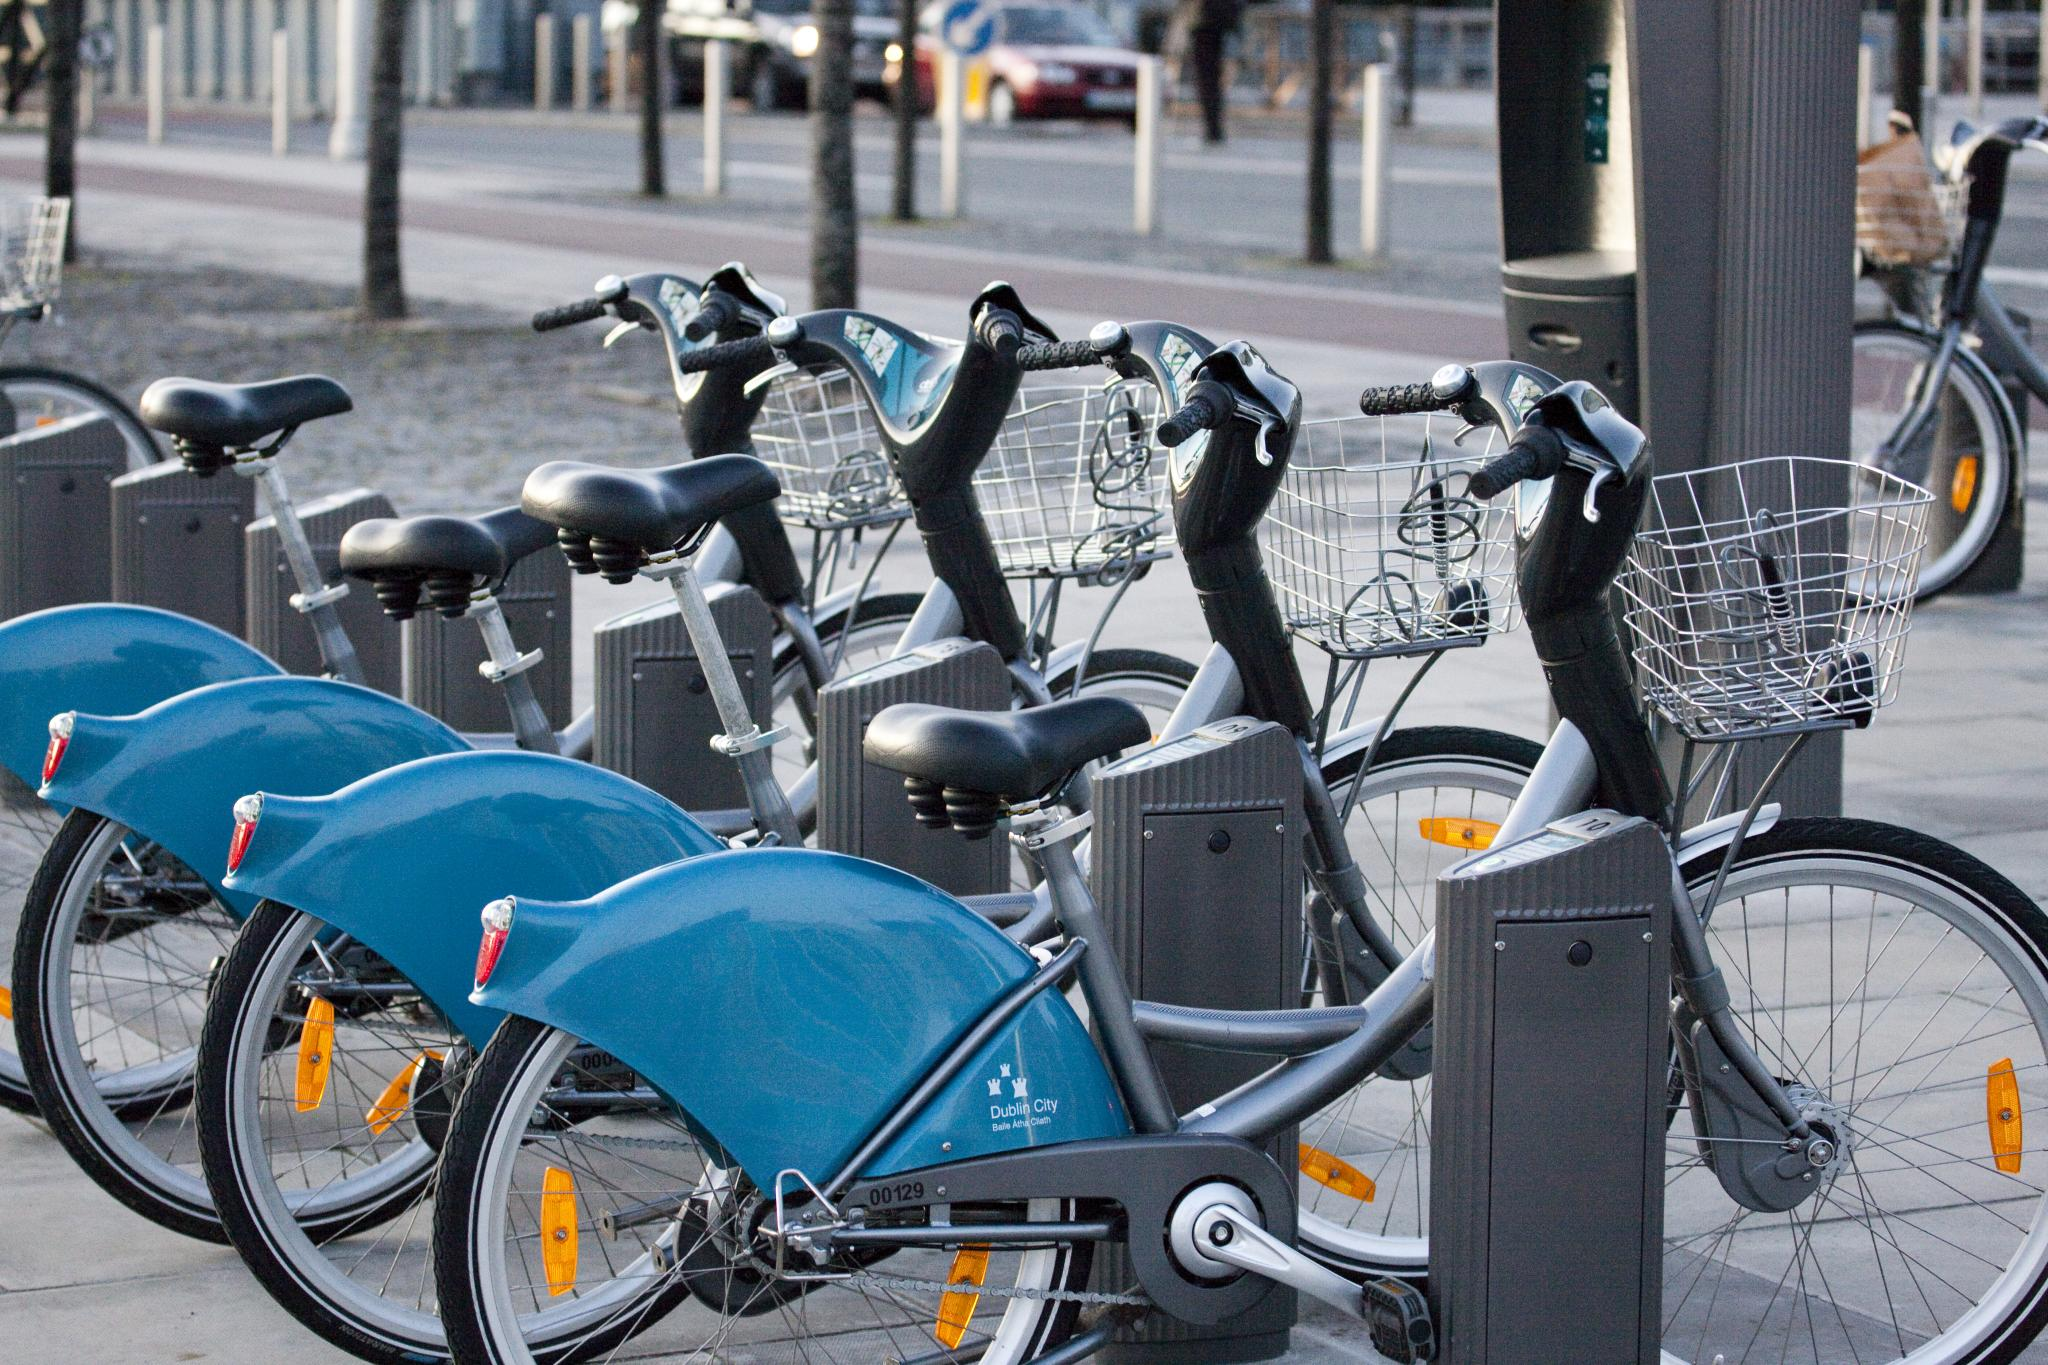
\includegraphics[width=\paperwidth]{db.jpg}};
\end{tikzpicture}

\restoregeometry   
\newpage


\vspace{-0.5cm}
\section{Introduction}
\vspace{-0.5cm}

The Dublin Bikes system was launched by the public transportation operator, Dublin Bus, in 2009 and has since become a popular and integral part of Dublin's transportation network. The system allows users to rent bikes from various stations located throughout the city for short trips, typically lasting less than 30 minutes. The bikes are widely used by commuters, tourists, and residents alike, providing a convenient and eco-friendly mode of transportation in the city. Today, the grid consists of 115 stations and around 1500 bicycles, and it has over 40 thousand registered users, with millions of trips taken annually\footnote{Smart Dublin. (2022, June 27). \textit{Dublin Bikes}. Retrieved April 19, 2024, from \url{https://smartdublin.ie/dublin-bikes/}}. This report presents the results of a data-based analysis to evaluate whether expanding or reducing the capacity of certain Dublin Bikes stations could improve the grid, enhancing efficiency and improving user experience.

\vspace{-0.5cm}
\section{Methodology}
\vspace{-0.5cm}

\vspace{0.3cm}
\noindent
To answer these questions, data on bike and stand availability of the Dublin Bikes grid was used, focusing on two key metrics to evaluate how well the grid works and how a proposed alternative grid could outperform the current one. First, the bike availability ratio for each station was considered. This ratio equals the number of available bikes over the number of total bike stands at each station at each point in time, and it tells us how empty or full each station is at any given observation. Second, the variance of this ratio was also key to the analysis. This number tells us whether the station is low or high in usage. Together, these metrics helped us identify problematic stations that should be reduced or expanded\footnote{Note that the problem was simplified to reducing/expanding current stations for simplicity, but this could easily be translated into eliminating stations rather than reducing them, and into creating new ones close to the ones that were deemed good candidates for expansion}. There are four possible combinations of ratio and variance values, which each signal different types of problems: 

\vspace{0.3cm}
\noindent First, a low ratio and low variance on a station tells us that the station is low on available bikes, but that the usage is quite low anyway. Although this is not the biggest concern because bikes are not being wasted at a station that is not very busy, the stations require maintenance and represent unnecessary costs, so these could be significantly reduced. Second, a high ratio and low variance signals that there are lots of available bikes in the station, although the station is not busy. This is arguably the worst problem: bikes that could be used elsewhere are parked here, in a station that people do not use. Thirdly, a low ratio and high variance signals that a station is quite busy, but bikes are not available. Expanding these stations to be equipped with enough bikes before these busy times could thus be very helpful and enhance user experience significantly. Finally, a high ratio and high variance is a sign that a busy station is full, and perhaps more people would like to park their bikes there, but they are not able to, so expanding these stations could be beneficial. These cases are further illustrated in Table 1 below. 

\begin{table}[h]
\centering
\caption{Explanation of problems for each combination of ratio and variance}
\begin{tabular}{|l|l|p{5cm}|p{5cm}|}
\hline
\multicolumn{2}{|c|}{} & \multicolumn{2}{c|}{\textbf{Variance}} \\
\cline{3-4}
\multicolumn{2}{|c|}{} & \textbf{Low} & \textbf{High} \\
\hline
\multirow{2}{*}{\textbf{Ratio}} & \textbf{Low} & Low usage; unnecessary maintenance cost of station. & Busy station with not enough bikes. \\
\cline{2-4}
& \textbf{High} & Low usage station with many bikes that could be better used elsewhere. & Busy station that is full and has no space for parking more bikes. \\
\hline
\end{tabular}
\label{tab:problem_explanation}
\end{table}

\noindent To account for the fact that usage may vary considerably depending on the time of the day due to the patterns that commuting and rush hours create, the ratio of available bikes was calculated for three different time slots, while the variance was calculated for the complete dataset (to measure how used bikes are). Specifically, a subset of the data was created to exclude observations that occur between 8 pm and 5 am, and then three time slots were created: the first one, ranging from 5 am to 10 am captures the morning rush hour patterns, the second one, from 10 am to 4 pm captures the time where people are at work, and the last one, from 4 pm to 8 pm captures the afternoon rush hour \footnote{The reason for this first filtering is that the Dublin Bikes are closed from 12:30 am to 5 pm, and the hours between 8 pm and 12:30 am were deemed not so relevant to the patterns that people's day to day routines create. In addition, the data that supported the analysis was also cleaned of weekend observations, as weekdays were deemed more important for the functioning of the grid and for studying patterns.}. 

\vspace{0.3cm}
\noindent In sum, these two metrics allow to identify problematic stations \textemdash stations where more or less bikes and/or more or less stands are needed to optimise the grid\textemdash. If our proposals of expansions and reductions of these stations are good, we should observe that the optimised grid contains less problematic stations. Thus, by calculating these metrics and sorting, we selected 20 bike stations that should be modified. We proposed that 10 of these be reduced in size, while the other half should be expanded, based on the type of problem case for each station. To evaluate our proposal, we used Machine Learning and created a simulation of the new grid with these changes to compare it to the current grid. First, we defined our target variable as a binary indicator that simply says whether the station is problematic or non-problematic. This was based on our definition of problematic stations presented above, and we used the following cutoffs to define problematic cases: 

\begin{table}[h]
    \centering
    \caption{Problem Indicators based on Availability Ratio and Ratio Variability}
    \begin{tabular}{|c|c|c|}
    \hline
    \textbf{Availability Ratio} & \textbf{Ratio Variability} & \textbf{Problem Indicator} \\
    \hline
    Less than 0.4 & Less than 4 & Problematic "low, low" \\
    Less than 0.4 & More than 7 & Problematic "low, high" \\
    More than 0.6 & Less than 4 & Problematic "high, low" \\
    More than 0.6 & More than 7 & Problematic "high, high" \\
    \hline
    \end{tabular}
    \label{tab:problem_indicators}
\end{table}

The following maps further show the standardised availability ratios and variance for the stations in the Grand Canal Dock area. Darker colors represent very high or very low values for both measures, and the circled marker is an example of a problematic station: this station has extreme values for both availability ratios and their variability. This snapshot is from the afternoon time slot. 

\begin{figure}[h]
    \centering
    \caption{Snapshot showing extreme values for ratio and variance metrics \\ (the map on the left shows ratios, the map on the right shows variance)}
    \includegraphics[width=\textwidth]{sections/map.png}
    \label{fig:example}
\end{figure}

\newpage
\noindent We then fit a binary K Nearest Neighbors classifier to predict whether a station is problematic or not, based on two features. The first feature is the cluster the station belongs to. We used k-means clustering on our data to group all the stations in the grid into 20 clusters, so that we could have a "proxy" of location that we could use as a feature, since, from the data visualisation process, we saw that both ratio and availability in stations tends to be similar for neighboring stations. The second feature is the time of the day, because during the data visualisation and exploration process we also learned that a station's ratio of available bikes can vary a lot depending on the time of the day. 

\vspace{0.3cm}
\noindent Finally, we ran a simulation where we made the changes we proposed for the stations. We made the necessary reductions and increases in the sizes of the selected stations (by 50\%, in both cases, for simplicity), we used our model to predict whether the station is problematic or not, and, finally, to evaluate our proposal we compared the predicted proportion of problematic stations in the original grid, compared to the new, optimized grid from the simulation. 

\vspace{-0.5cm}
\section{Results}
\vspace{-0.5cm}

\noindent The results from fitting the classifier indicate that the dataset is balanced, with similar counts of samples categorised as problematic and non-problematic in both the original and simulated datasets. Specifically, the original dataset consists of 172,188 problematic instances and 168,253 non-problematic instances, while the simulated dataset comprises 170,400 non-problematic instances and 170,041 problematic instances.

\vspace{0.3cm}
\noindent As for the Machine Learning model performance, the accuracy for both the original data and the simulation is around 65\%, and the confusion matrices reveal that the algorithm performs better when identifying non-problematic instances, while it struggles with spotting problematic ones. While the model's performance could be improved, the fact that it is consistent across both datasets means that the proposal can still be correctly evaluated. 

\vspace{0.3cm}
\noindent After fitting the model for the original grid and then repeating the process for the simulation data, the proportion of problematic stations did decrease. The following Figure 2 shows this change for two of the clusters that the stations were grouped into. In the ninth cluster, the proportion of problematic stations went from 0.5 to 0.33, and in the sixteenth cluster this figure changed from 0.33 to 0.16. 

\begin{figure}[h]
    \centering
    \caption{Proportion of problematic bike stations before and after optimisation for two clusters}
    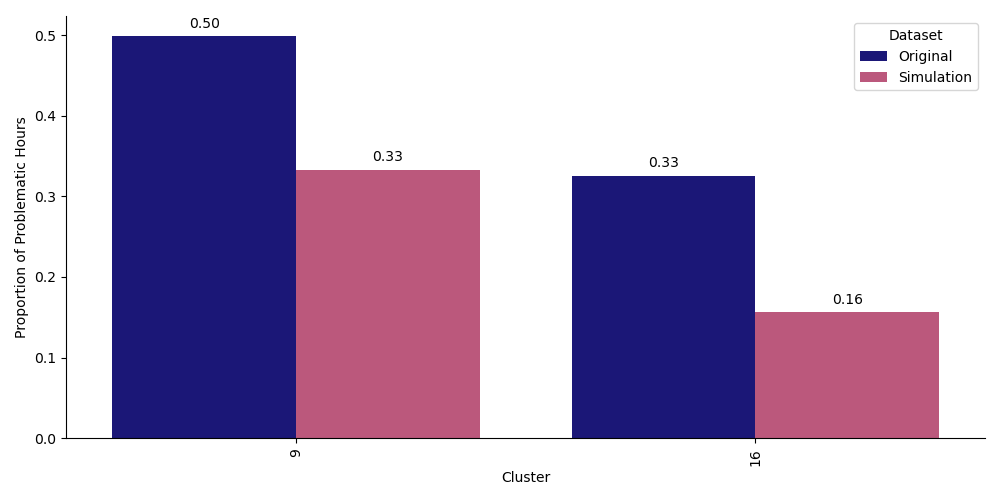
\includegraphics[width=\textwidth]{sections/res3.png}
    \label{fig:example}
\end{figure}

\vspace{-1cm}
\section{Conclusions}
\vspace{-0.5cm}

In sum, this analysis of the Dublin Bikes system aimed to optimise its grid for enhanced efficiency and user experience. By evaluating bike and stand availability metrics, problematic stations were identified, informing proposals for the expansion and reduction of stations. These proposals were assessed using machine learning techniques, revealing consistent performance across original and simulated datasets despite moderate performance of the Machine Learning algorithm for predictions. The simulation results indicate that the proposed changes could lead to a reduction in the proportion of problematic bike stations. Overall, while the model's performance could be refined, the findings provide valuable insights for optimising the Dublin Bikes system, potentially improving its functionality and user satisfaction, as well as helping to cut unnecessary costs. 

\setlength{\itemsep}{-0.2cm}
\setlength{\parsep}{-0.2cm}

\end{document}